\chapter{Nasadenie do vyučovania}
\label{chap:nasadenie_do_vyucovania}

Aby bola preverená celková kvalita a využiteľnosť virtuálneho laboratória, bol nástroj EVE-ng nasadený na vypracovávanie rôznych topológii z vybraných predmetov, ktoré sú opísané v nasledujúcich častiach tejto kapitoly. Zároveň budú popísané aj problémy, ktoré proces nasadzovania sprevádzali. Predmety sú uvedené v poradí podľa toho, v akom čase bol nástroj EVE-ng na nich používaný. Návod na vytvorenie vlastnej topológie je uvedený v kapitole \ref{chap:pouzivanie_eve_ng}.





\section{Projektovanie sietí 2}

V rámci predmetu Projektovanie sietí 2 bol nástroj EVE-ng nasadený do vyučovania na vypracovávanie topológii s pokročilejšími sieťovými technológiami. Topológie boli spustené na virtuálnom EVE-ng serveri.

V EVE-ng boli úspešne dokončené semestrálne práce zamerané na pokročilé technológie v témach z oblastí \emph{VPLS} a \emph{Seamless MPLS}. Téma \emph{EVPN} bola vypracovávaná v nástroji \emph{ViRo2}.

Topológie semestrálnych prác sa skladali z týchto zariadení:

\begin{itemize}[noitemsep]
    \item Cisco IOL smerovač - VPLS, Seamless MPLS
    \item Cisco CSR - VPLS
    \item Juniper Olive 12.1 - Seamless MPLS
    \item Juniper vMX 15 - VPLS
    \item Nokia VSR - EVPN
\end{itemize}

Vypracovávanie semestrálnych prác sa však nezaobišlo bez komplkácii. Neustále bola zapracovávaná spätná väzba študentov pracujúcich v skupinách ohľadom používania nástroja EVE-ng a podporovaných technológii zariadení. Zistilo sa napríklad, že virtuálna inštalácia EVE-ng neposkytuje dostatočný výkon, ktorý bol potrebný na vypracovanie všetkých semestrálnych prác. Preto bol vytvorený fyzický EVE-ng server, ktorý bol nasadený na nasledujúcom predmete, Počítačové siete 2. Fyzický server vykazoval vyšší výkon v porovnaní s virtuálnym, čo mohlo byť s veľkou pravdepodobnosťou spôsobené dodatočným hypervízorom VMware pri virtuálnom serveri.





\section{Počítačové siete 2}

V rámci predmetu Počítačové siete 2 bol nástroj EVE-ng nasadený do vyučovania na vypracovávanie topológii s \emph{point-to-point} technológiami. Topológie boli spustené na fyzickom EVE-ng serveri. V prípade zlyhania EVE-ng boli pripravené aj záložné topológie v nástroji Dynamips/Dynagen.

Najprv bola vytvorená základná topológia, znázornená na obrázku \ref{obr:eve_ng_ppp_zakladna_topo_v2}. Tá pozostávala zo štyroch Cisco IOL smerovačov a dvoch koncových zariadení s operačným systémom Alpine Linux. Cisco IOL smerovač bol vybraný, pretože ako jediný podporoval sériové rozhrania a \emph{point-to-point} technológie. Koncové zariadenie Alpine Linux bolo vybrané pre svoju nenáročnosť na systémové zdroje.

Celkovo bolo vytvorených 8 zhodných topológii, ktoré medzi sebou zdieľali jeden učiteľský smerovač. V topológii sa celkovo nachádzalo 33 Cisco IOL smerovačov a 16 koncových staníc. Celková topológia sa nachádza na obrázku \ref{obr:eve_ng_ppp_celkova_topo_v2}.

\begin{figure}
    \centering
    \includegraphics[width=0.6\textwidth,trim={2cm 0cm 2cm 2.5cm},clip]{eve_ng_ppp_zakladna_topo_v2}
    \caption{Základná PPP topológia}
    \label{obr:eve_ng_ppp_zakladna_topo_v2}

    \vspace{3cm}

    \centering
    \includegraphics[width=1.0\textwidth,trim={4cm 10cm 0.5cm 4cm},clip]{eve_ng_ppp_celkova_topo_v2}
    \caption{Celková PPP topológia}
    \label{obr:eve_ng_ppp_celkova_topo_v2}
\end{figure}

IOL smerovače fungovali, až na príkaz \texttt{clock rate} na sériových rozhraniach, bez chyby. Ukázalo sa, že nastavenie DCE/DTE závisí od párnosti čísla skupiny. Párne číslo skupiny sériových rozhraní bude vždy DTE, nepárne vždy DCE, ako je zrejmé z obrázku \ref{obr:eve_ng_dce_dte_2E8S}. Rozdelenie sériových rozhraní na DCE/DTE nezávislé od počtu ethernetových alebo sériových skupín, čo potvrdzuje obrázok \ref{obr:eve_ng_dce_dte_1E8S}. Nastavenie DTE/DCE módu pre sériové rozhrania je v EVE-ng pri Cisco IOL smerovačoch pevne dané a nedá sa zmeniť, na čo treba myslieť pri návrhu topológie. Pre porovnanie, v nástroji Dynamips/Dynagen sa dá DCE/DTE mód na jednotlivých sériových rozhraniach ľubovoľne meniť.

\begin{figure}
    \centering
    \includegraphics[width=0.7\textwidth]{eve_ng_dce_dte_2E8S}
    \caption{Typy sériových rozhraní na IOL smerovači - 2 ethernetové + 8 sériových skupín}
    \label{obr:eve_ng_dce_dte_2E8S}

    \vspace{1cm}

    \centering
    \includegraphics[width=0.7\textwidth]{eve_ng_dce_dte_1E8S}
    \caption{Typy sériových rozhraní na IOL smerovači - 1 ethernetová + 8 sériových skupín}
    \label{obr:eve_ng_dce_dte_1E8S}
\end{figure}

V jednej študentskej skupine sa vyskytol problém s jednosmernou PAP autentifikáciou študentského smerovača voči učiteľskému (R\_Ucitel(s4/1)-5R2(s2/1)). Príkaz \\\texttt{debug ppp authentication} hlásil chybu pri autentifikácii. Riešenie spočívalo v odstránení používateľa, vypnutí \emph{ppp} konfigurácie a vypnutí rozhraní. Všetky tieto kroky boli vykonané aj na učiteľskom, aj na študentskom smerovači. Následne sa konektivita obnovila a spojenie pomocou PAP autentifikácie sa úspešne nadviazalo.

Je možné, že problémy vznikli aj kvôli tomu, že medzi študentským a učiteľským smerovačom boli na oboch stranách sériové rozhrania párnej skupiny t.j. obidva konce linky boli typu DTE. Niektoré skupiny študentov boli tiež pripojené k učiteľskému smerovaču sériovým rozhraním z párnej skupiny, ale takéto problémy nezaznamenali. Podobne tomu bolo aj pri prepojení Cisco IOL smerovačov rozhraniami DCE.

Z toho vyplýva, že Cisco IOL smerovače v EVE-ng majú pri prepojení dvoch smerovačov sériovou linkou s rovnakým módom nedefinované správanie. Tomu sa dá predísť vhodným návrhom topológie. Ten spočíva v tom, že sériové rozhrania medzi smerovačmi kombinujeme tak, aby bolo prepojené vždy sériové rozhranie párnej skupiny na jednom smerovači so sériovým rozhraním nepárnej skupiny na inom smerovači t.j. \emph{Serial2/x} (DCE) na prvom smerovači sa musí pripojiť napr. k \emph{Serial3/x} na druhom. V takom prípade DCE koniec po nastavení \texttt{clock rate} v príkaze \texttt{show controllers} zobrazí nastavený atribút \emph{received clockrate}, DTE koniec naproti tomu zobrazí hodnotu \emph{n/a}. Napriek tomu konektivita po správnom nastavení IP adries a zapnutí rozhraní bola aktívna.

Komplikácie s DCE/DTE a PPP autentifikáciou boli prítomné v prvom návrhu topológie, ktorý je znázornený na obrázku \ref{obr:eve_ng_ppp_zakladna_topo_v1}.

Pri testovaní DCE/DTE rozhraní sme narazili na obmedzenie nástroja EVE-ng. Community verzia je totiž dovoľuje v jednej topológii mať spustených najviac 63 zariadení. Po spustení 64. sa na niekoľko sekúnd spustí, ale nakoniec sa automaticky vypne. Community verzia vie spustiť aj viac ako 64 zariadení v jednej topológii, ale vo výsledku sa spustia len niektoré, na prvý pohľad náhodne vybrané zariadenia. Avšak tie zariadenia, ktoré sa spustia, pracujú štandardným spôsobom. Uvedený problém sa nám nepodarilo vyriešiť ani rozšírením rozsahu portových čísel pre zariadenia v topológii.
  
Zmerané boli aj systémové požiadavky celkovej topológie na fyzickom EVE-ng serveri. Po vyhodnotení výsledkov merania sme zistili, že celá topológia, 33 Cisco IOL smerovačov a 16 koncových zariadení Alpine Linux, sa spúšťala približne 2 minúty, spotrebovala 13GB operačnej pamäte a procesor vyťažovala na 21\%. Celkovo by sme podľa celkového vyťaženia CPU mohli spustiť 4 takéto topológie, avšak množstvo operačnej pamäte by dovoľovalo spustiť iba 3. Tabuľkový dokument s výsledkami merania systémových požiadaviek topológie je prítomný v kapitole \ref{chap:cd} v bode \ref{item:nasadenie_ps2_benchmark}

\begin{figure}[htbp]
    \centering
    \includegraphics[width=0.5\textwidth,trim={12cm 2cm 23.7cm 7cm},clip]{eve_ng_ppp_zakladna_topo_v1}
    \caption{Základná PPP topológia - prvotný návrh}
    \label{obr:eve_ng_ppp_zakladna_topo_v1}
\end{figure}

Spomenutý súbor ukazuje veľké rozdiely v meraniach využitia operačnej pamäte medzi nástrojmi \emph{ps} a \emph{ps\_mem} v hárku \emph{VstupVystup}, hoci sa merala rovnaká množina procesov. Po manuálnom overení sa ukázalo, že prvý menovaný nástroj vykazoval presnejšie výsledky, preto boli pri odhadoch použité ním namerané hodnoty.

Študenti počas vypracovávaní topológie na predmete Počítačové siete 2 nezaznamenali žiadny rozdiel oproti nástroju Dynamips/Dynagen, keďže sa na zariadenia prihlasovali rovnako, pomocou nástroja \emph{PuTTY} IP adresou a portom, pričom zariadenia poskytovali, až na malé výnimky rovnaké funkcie, ako v nástroji Dynamips/Dynagen. Nástroj EVE-ng na fyzickom serveri bol počas celej doby vypracovávania stabilný. Zariadenia boli počas celého vyučovania spustené a samovoľne sa nevypínali. Fyzický EVE-ng server je tým pádom vhodný na používanie na predmete Počítačové siete 2.






\section{Projektovanie sietí 1}

V rámci predmetu Projektovanie sietí 1 bol nástroj EVE-ng nasadený do vyučovania na vypracovanie topológií na tému \emph{MPLS}. V prípade zlyhania EVE-ng boli pripravené aj záložné topológie v nástroji Dynamips/Dynagen.

Najprv bola stanovená základná topológia (obr. \ref{obr:mpls_zakladna_topo}). Od nej sa odvíjali ostatné topológie. Celkovo bolo použitých týchto 6 typov zariadení:

\begin{itemize}[noitemsep]
    \item Cisco IOL prepínač
    \item Cisco IOL smerovač
    \item Cisco 3725 smerovač (Dynamips) s EtherSwitch modulom
    \item Cisco 7200 smerovač (Dynamips)
    \item Cisco vIOS smerovač (QEMU)
    \item Cisco vIOS prepínač (QEMU)
\end{itemize}

Topológie pozostávali z 10 Cisco smerovačov resp. Cisco MLS. Z každého typu boli spustené 2 topológie t.j. 20 zariadení, okrem Cisco vIOS a vIOS L2 prepínača, z ktorých bola vytvorená iba jedna pre každý typ. 

Rôzne zariadenia sa použili preto, aby boli otestované funkcie ich jednotlivých typov. Pokiaľ by sa ukázalo, že viaceré zariadenia podporujú nutné technológie, môžeme v budúcnosti použiť iba tie, ktoré vyžadujú najmenšie systémové prostriedky. Tak sa dá maximalizovať množstvo spustených zariadení.


\begin{figure}
    \centering
    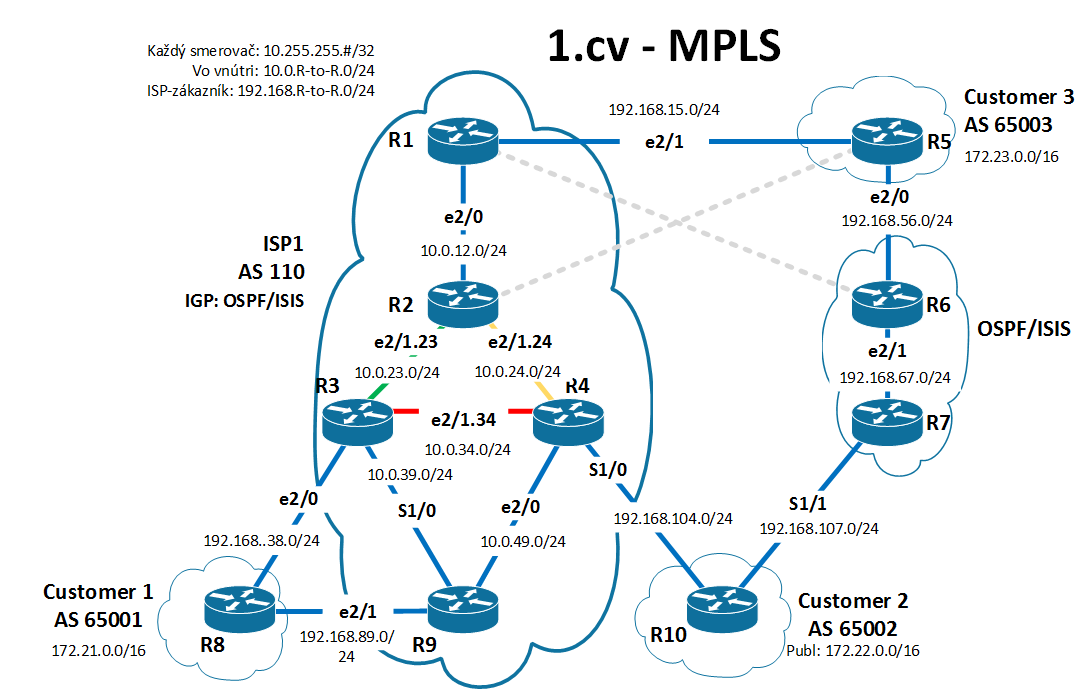
\includegraphics[width=1\textwidth,trim={0cm 0cm 0cm 0cm},clip]{mpls_zakladna_topo}
    \caption{Základná MPLS topológia}
    \label{obr:mpls_zakladna_topo}
    \cite{mpls_zakladna_topo}
\end{figure}

Celkovo bolo v topológii spustených 40 Dynamips zariadení, 40 IOL zariadení, a 20 QEMU zariadení. Vyťaženie procesora sa pohybovalo medzi 35-65\%, pričom bolo využitých približne 28 GB operačnej pamäťe.

Študenti boli rozdelení do 10 skupín po dvoch študentoch. Z toho vyplýva, že bolo potrebné spustiť najmenej 10 topológii t.j. celkovo 100 zariadení.

Avšak EVE-ng vo verzii \emph{Community} dokáže v jednej topológii stabilne spustiť najviac 63 zariadení. Preto boli vytvorené dva používateľské účty s rolou \emph{editor}. V oboch účtoch bolo vytvorených 6 topológii, pre každý typ zariadenia jedna. Pre spomenuté používateľské účty bol vybraný taký \emph{POD} identifikátor, aby sa portový rozsah začínal číslom 1, aby to zodpovedalo názvu smerovača prvého smerovača, R1. Zvolené identifikátory boli \emph{9} pre prvého a \emph{14} pre druhého používateľa.

Topológie boli vytvárané tak, aby bol zachovaný počet zariadení a ich prepojenia medzi nimi. Avšak názvy rozhraní rôznych typov zariadení neboli vždy rovnakého typu alebo neboli rovnako očíslované. Preto boli rozhrania pre jednotlivé typy zariadení vybrané tak, aby logicky podľa jednoduchého pravidla zodpovedali tým v pôvodnej topológii. Napr. Cisco IOL zariadenia mali 3 skupiny \emph{Ethernet} rozhraní namiesto dvoch, aby sa názvy rozhraní zhodovali s pôvodným návrhom MPLS topológie (e2/x).

Súčasťou topológie je aj \emph{bridge} zariadenie, ktorého úlohou je iba vytvoriť \emph{broadcast} doménu medzi smerovačmi R2, R3 a R4 a preposielať v rámci nej rámce. Výhodou takéhoto zariadenia sú minimálne požiadavky na systémové prostriedky, keďže po jeho vytvorení sa vytvorený iba \emph{bridge} rozhranie na serveri.

Každému študentovi bol vytvorený používateľský účet s rolou \emph{user}. Tento účet mal slúžiť na prehliadanie topológie priradenej danej skupine. V momente, keď sa študenti začali prihlasovať do webového rozhrania EVE-ng a začali otvárať potrebné súbory s topológiami, server v dôsledku tejto záťaže vykazoval maximálne vyťaženie a stal sa nestabilným. Nestabilita bola vyriešená ukončovaním výpočtovo náročných procesov pomocou vzdialeného prístupu cez SSH. Ukázalo sa, že otváranie topológie je v nástroji EVE-ng výpočtovo náročná činnosť Tomuto problému sa dá predísť tak, že topológie budú jednotliví používatelia otvárať postupne, jeden po druhom. Pri sledovaní záťaže počas otvárania topológie server vykazoval vyššiu záťaž, ktorá sa po dokončení načítavania ustálila.

Nakoniec si všetci študenti otvorili príslušné súbory s topológiou, aby videli, ktoré rozhrania je potrebné jednotlivým zariadeniam konfigurovať. Súbory s topológiou slúžili ako doplnok ku pôvodnému návrhu topológie, ktorý obsahoval dodatočné informácie, ako sú adresácia a čísla autonómnych systémov pre BGP.

Žiaľ, študenti nevypracovali topológiu na tému MPLS v nástroji EVE-ng, pretože dokončovali úlohy z predchádzajúcich cvičení.




\section{Vyhodnotenie}

Z predmetov Počítačové siete 1, Pokročilé prepínanie v informačno-komunikačných sieťach a Pokročilé smerovanie v informačno-komunikačných sieťach neboli vypracované žiadne topológie.

Na predmetoch, kde nástroj EVE-ng nasadený bol, sa ukázalo, že ho je možné používať vo vyučovaní.

Pri nasadení na predmet Projektovanie sietí 2, kde bola použitá virtuálna inštalácia EVE-ng, bol naopak nástroj nestabilný, zariadenia často zamŕzali a pri zadávaní príkazov do konzoly bola prítomná vyššia odozva z klávesnice. Mohlo to byť spôsobené mnohými faktormi, či už samotnou virtuálnou platformou VMware, alebo nesprávne nastavenými systémovými parametrami pre jednotlivé zariadenia v topológii.

Napriek mnohým nedostatkom nástroja EVE-ng, je minimálne pre učiteľov výhodou, že môžu vytvárať topológie z grafického rozhrania, namiesto z príkazového riadku. Nevýhodami sú nemožnosť stabilne spúšťať viac ako 63 zariadení v jednej topológii. Jednotliví používatelia a študenti si svoje topológie nemôžu spravovať nezávisle na sebe, keďže toto je možné iba v Learning Centre verzii nástroja, ktorá súbory jednotlivých používateľov od seba oddeľuje.

Čo sa týka odhadov systémových požiadaviek topológii, tie môžeme odhadnúť súčtom systémových požiadaviek jednotlivých zariadení, ktoré sa v topológii budú nachádzať. Systémové požiadavky vybraných zariadení sú k dispozícii na CD v kap. \ref{chap:cd} v bode \ref{item:all_benchmarks} Tak môžu byť vopred odhadnuté systémové požiadavky konkrétnej topológie.

Z meraní systémových požiadaviek celých topológií z predmetov Počítačové siete 2 a Projektovanie sietí 1 vyplýva, že namerané systémové požiadavky zariadení uvedené v kap. \ref{chap:cd} v bode \ref{item:all_benchmarks} reprezentujú najhorší možný scenár a v skutočnosti fyzický EVE-ng server bude mať ešte dostatočnú výkonovú rezervu. Rezervu je možné pri homogénnej topológii kvantifikovať jednoduchšie, než pri topológiách s rôznymi druhmi zariadení.